\documentclass[a4paper, 12pt]{article}

% Packages
\usepackage[utf8]{inputenc}
\usepackage{amsmath}
\usepackage{geometry}
\usepackage{fancyhdr}
\usepackage{graphicx}
\usepackage{hyperref}
\usepackage{setspace}
\usepackage{indentfirst}
\usepackage{titlesec}
\usepackage{titling}
\usepackage{csquotes}
\usepackage{float}

% APA style citation package
\usepackage[style=authoryear-ibid, backend=biber, citestyle=authoryear-comp]{biblatex}
\addbibresource{references.bib}

% apa @ conestoga in line style
\DeclareCiteCommand{\parencite}
  {\usebibmacro{prenote}}
  {(\printnames{labelname}\addcomma\space\printdate}
  {\addcomma\space}
  {\usebibmacro{postnote})}

% Page Settings
\geometry{margin=2.54cm}
\doublespacing

% hyperlink setup
\hypersetup{
    hidelinks=true
}

% indentation
\setlength{\parindent}{1em}

% Define Heading Level 1 (centered, bold, title case)
\titleformat{\section} % Section = Heading Level 1
  {\centering\bfseries\Large} % Centered and bold
  {} % No section number
  {0pt} % No indent
  {} % No additional formatting for the title text

% Define Heading Level 2 (left-aligned, bold, title case)
\titleformat{\subsection} % Subsection = Heading Level 2
  {\bfseries\large} % Left-aligned and bold
  {} % No subsection number
  {0pt} % No indent
  {} % No additional formatting for the title text

% Define Heading Level 3 (left-aligned, bold & italic, title case)
\titleformat{\subsubsection} % Subsubsection = Heading Level 3
  {\bfseries\itshape\normalsize} % Left-aligned, bold, italic
  {} % No subsubsection number
  {0pt} % No indent
  {} % No additional formatting for the title text

% Define paper variables
\newcommand{\studentname}{Group 4: Isaiah Andrews, Joel Regi Abraham, Salah Salame, Jonathan Taylor}
\newcommand{\affiliation}{Applied Computer Science \& IT, Conestoga College}
\newcommand{\course}{CSCN 73060: Project VI: Software Efficiency and Performance}
\newcommand{\instructor}{Gurpreet Kaur}
\newcommand{\duedate}{\today}
\newcommand{\maintitle}{Performance Technical Report}
\newcommand{\subtitle}{\texttt{\textbf{libraryapi}}}

% Define a command to create the title page
\newcommand{\conestogatitlepage}{
    % \pagestyle{fancy}
    \thispagestyle{plain}
    \fancypagestyle{plain}{
        \fancyhf{}
        \renewcommand{\headrulewidth}{0pt}
        \fancyhead[R]{\thepage}
    }

    \vspace*{3\baselineskip}
    \begin{center}
        {\bfseries \maintitle \\ \subtitle}
        \vspace*{\baselineskip} \\
        \studentname \\
        \affiliation \\
        \course \\
        \instructor \\
        \duedate \\
    \end{center}
}

\pagestyle{fancy}
\fancyhf{}
\fancyhead[L]{\leftmark}
\fancyhead[R]{\thepage}

\begin{document}

% Title Page
\conestogatitlepage
\newpage

% Table of Contents
\tableofcontents
\newpage

\textbf{Abstract:}
\par Throughout this project, we developed a webserver using the CROW framework, and the C/C++ programming languages. The purpose
of this project was to evaluate performance under measured workloads and assess whether or not our system is performing adequately.
Our results show that initially, the root request had significant load since it fetched for all resources within our database, whereas
atomic operations (\texttt{POST}, \texttt{PUT}, \texttt{PATCH}, \texttt{DELETE}, \texttt{OPTIONS}) deal with a particular entry at a time.
To solve this, we implemented pagination, where only a fixed amount of resources can be gathered with a single \texttt{GET} request. This has shown
significant improvement in our response times and reduced the overall load on the server.

\section{Introduction}
\par Performance testing evaluates how a system will perform in terms of
stability and responsiveness under a particular workload. This project evaluates 
the role of performance testing within a production environment, where we measure the
threshold our system can handle and look for any ways of improvement.

\section{Test Design}
\par The testing for the webserver was conducted in Apache JMeter, covering each \enquote{verb} within our
API, and made use of graphs to better visualize the data.

\begin{itemize}
    \item \textbf{libraryapi\_TestPlan}
    \begin{itemize}
        \item $\downarrow$ \textbf{Thread Group}
        \begin{itemize}
            \item \texttt{Root} Request
            \item \texttt{POST\_Add\_Book}
            \item \texttt{PUT\_Update\_Book}
            \item \texttt{PATCH\_Redescribe\_Book}
            \item \texttt{DELETE\_Delete\_Book}
            \item \texttt{OPTIONS}
            \item Graph: Latencies Over Time
            \item Graph: Transactions per Second
            \item Results Tree
        \end{itemize}
    \end{itemize}
\end{itemize}

\subsection{API Design}
\par The webserver was implemented using the CROW framework, written in C/C++, where we made use of parametrized
URLs to both store and retrieve the right book at any given time. The WEB API was tested against a high volume of users
over a fixed interval of time.

\begin{table}[H]
    \centering
    \begin{tabular}{|l|l|l|}
        \hline
        \textbf{HTTP Verb} & \textbf{Route} & \textbf{Description} \\
        \hline
        \texttt{GET} & \texttt{/} & Displays all the books from the database \\
        \texttt{POST} & \texttt{/add} & Submit a new book record \\
        \texttt{PUT} & \texttt{/update/\{id\}} & Updates a book record by ID \\
        \texttt{PATCH} & \texttt{/redescribe/\{id\}} & Updates only the description field for a record by ID \\
        \texttt{DELETE} & \texttt{/delete/\{id\}} & Deletes a book record by ID \\
        \texttt{OPTIONS} & \texttt{/} & Displays the available verbs/routes of the web server \\
        \hline
    \end{tabular}
    \caption{HTTP API Endpoints}
\end{table}

\section{Results}

\par For the execution of performance test plan we used JMeter. Our test plan covered each verb that our API was configured to handle. \texttt{GET}, \texttt{POST}, \texttt{PUT}, \texttt{PATCH}, \texttt{DELETE}, \texttt{OPTIONS} and a request for the root URL.
Our test plan had two listeners to collect the test data and create graphical representations: Response Latency and Transactions per Second.

\par Our initial tests showed a significant deviation from our root request when compared to our other methods, where we conclude that since it is attempting to
access all the books stored within the database, the response times will be longer, and are directly tied to the amount of books we have to retrieve.

\par After adding pagination to the web-server, we were able to make the response times more consistent
by not querying all the books on record, and instead query a fixed amount at a time from our database.
This removes additional overhead on the webserver and allows for load-balancing on our resources for better
management.

\subsection{First Run}

\begin{figure}[H]
    \centering
    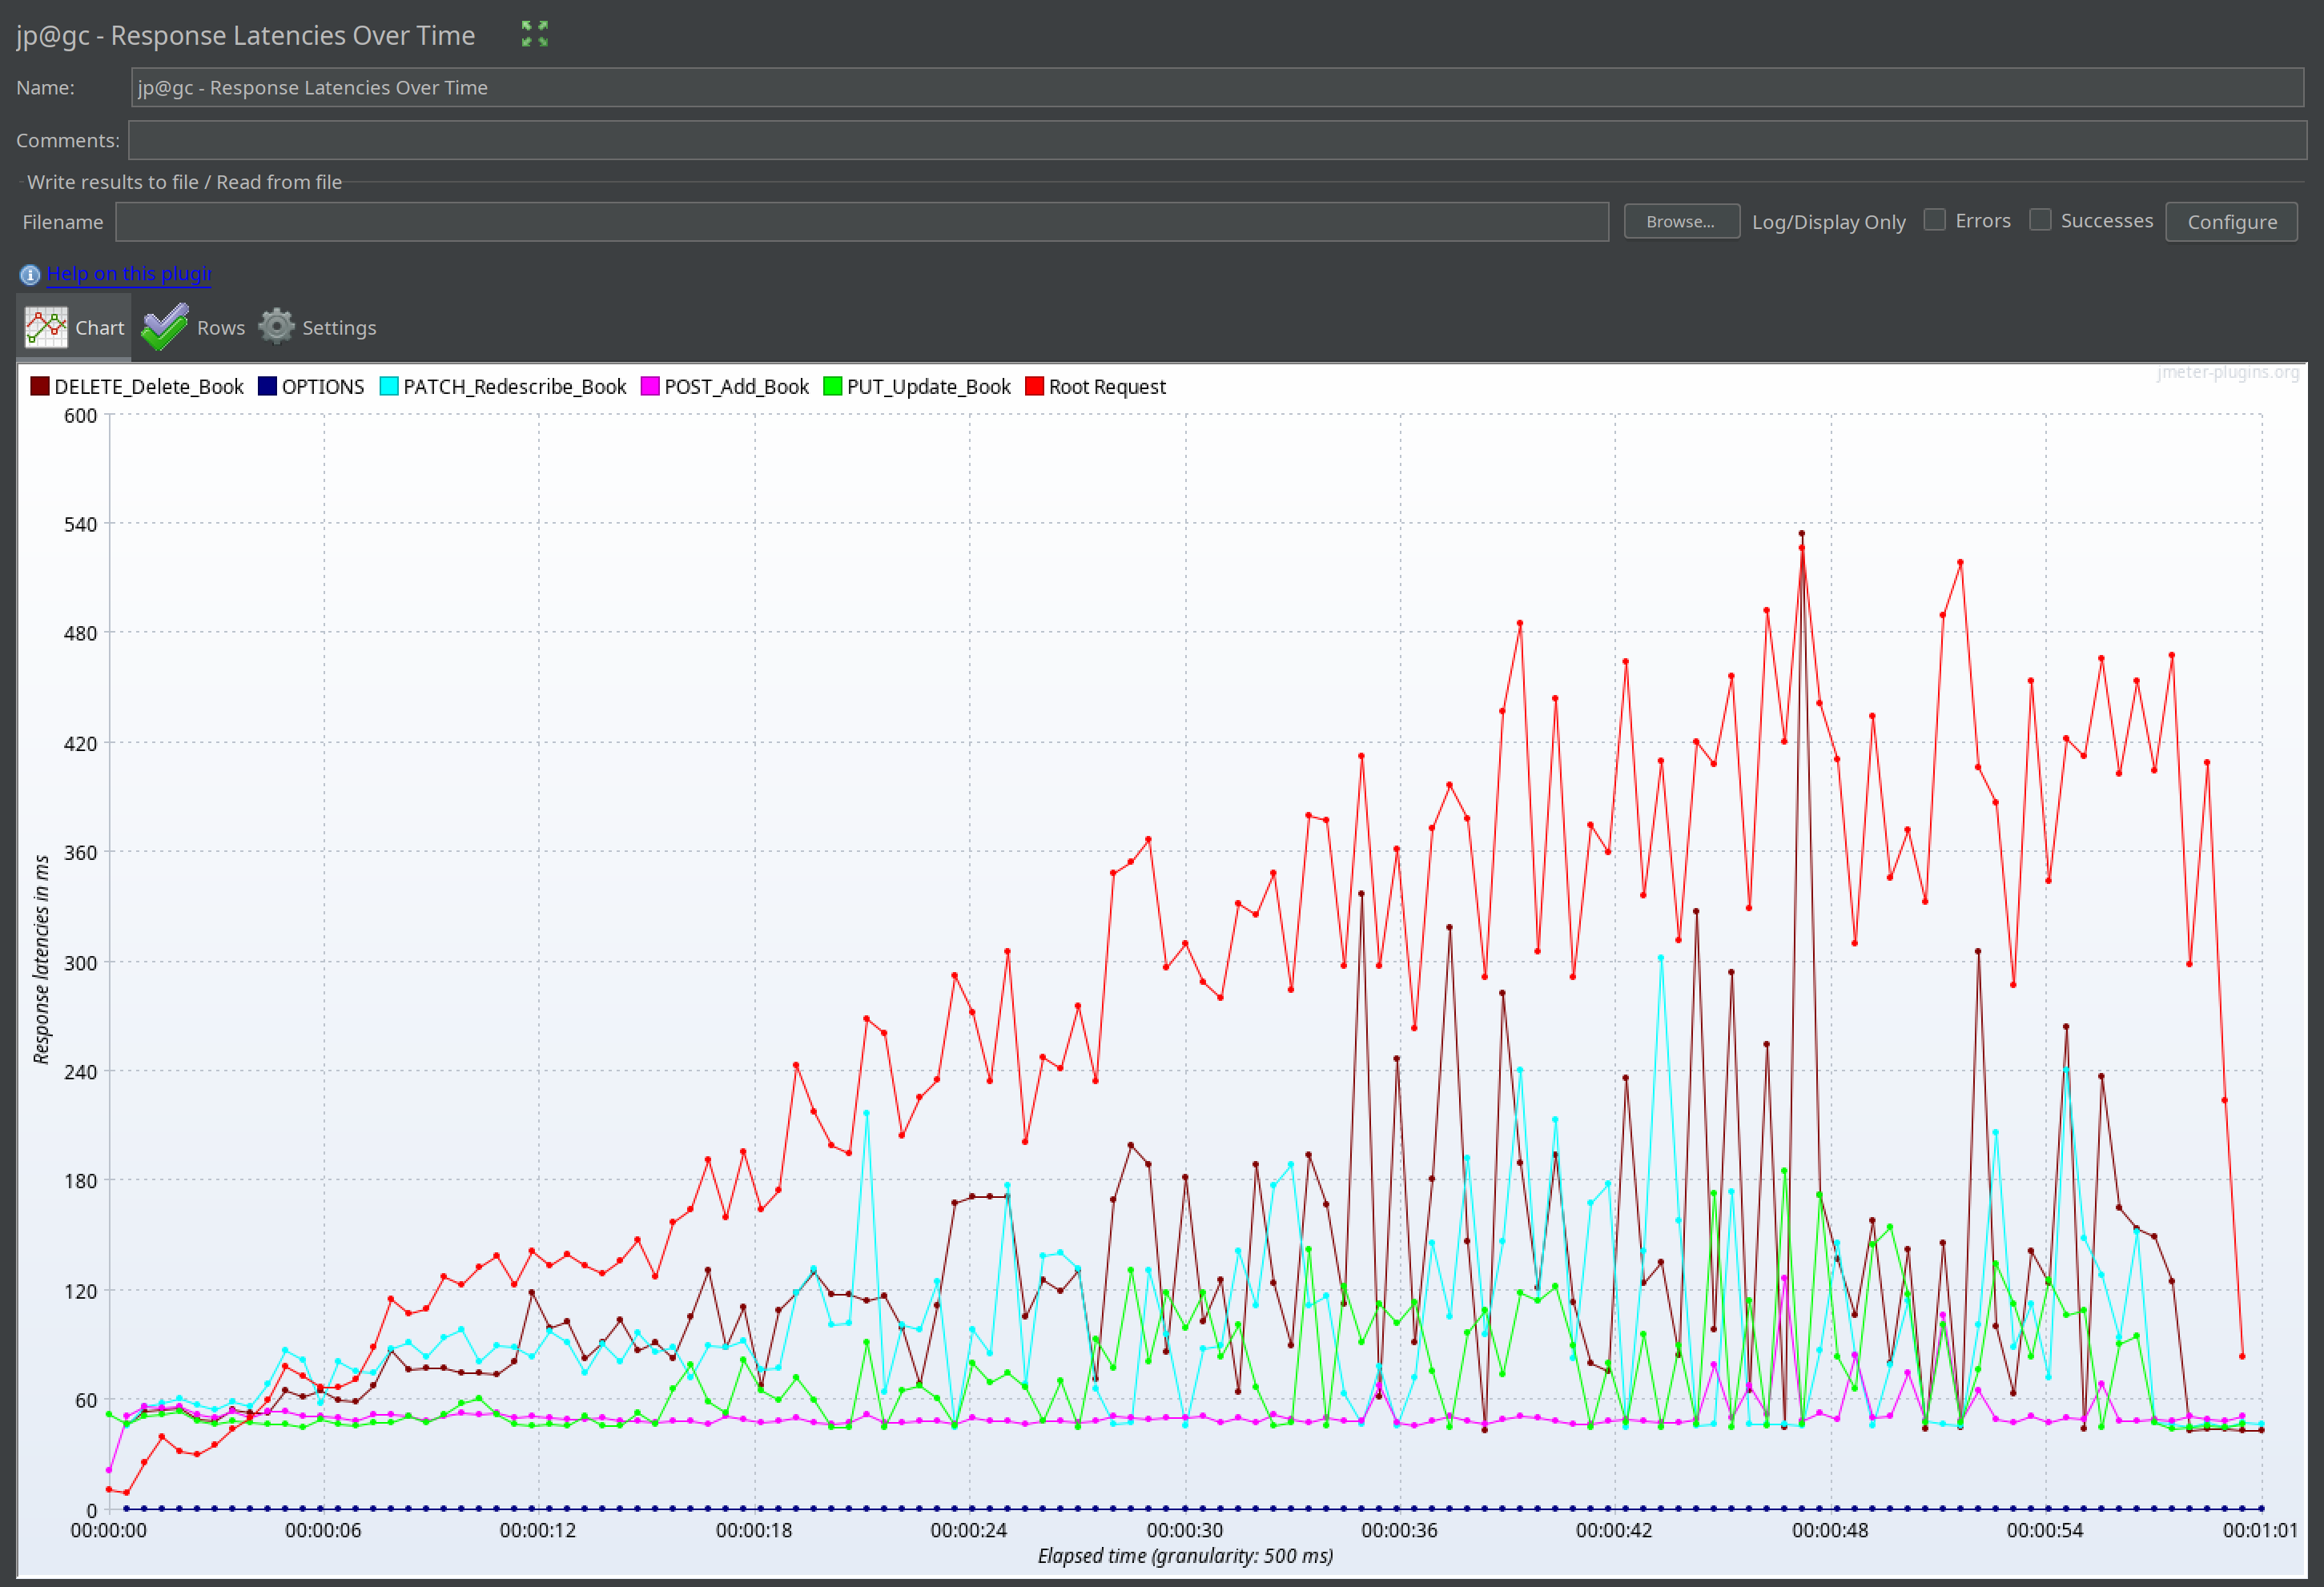
\includegraphics[width=0.65\textwidth]{../perfRuns/secondRunRespLatency.png}
    \caption{\textbf{Response Latency Graph}}
\end{figure}

\begin{figure}[H]
    \centering
    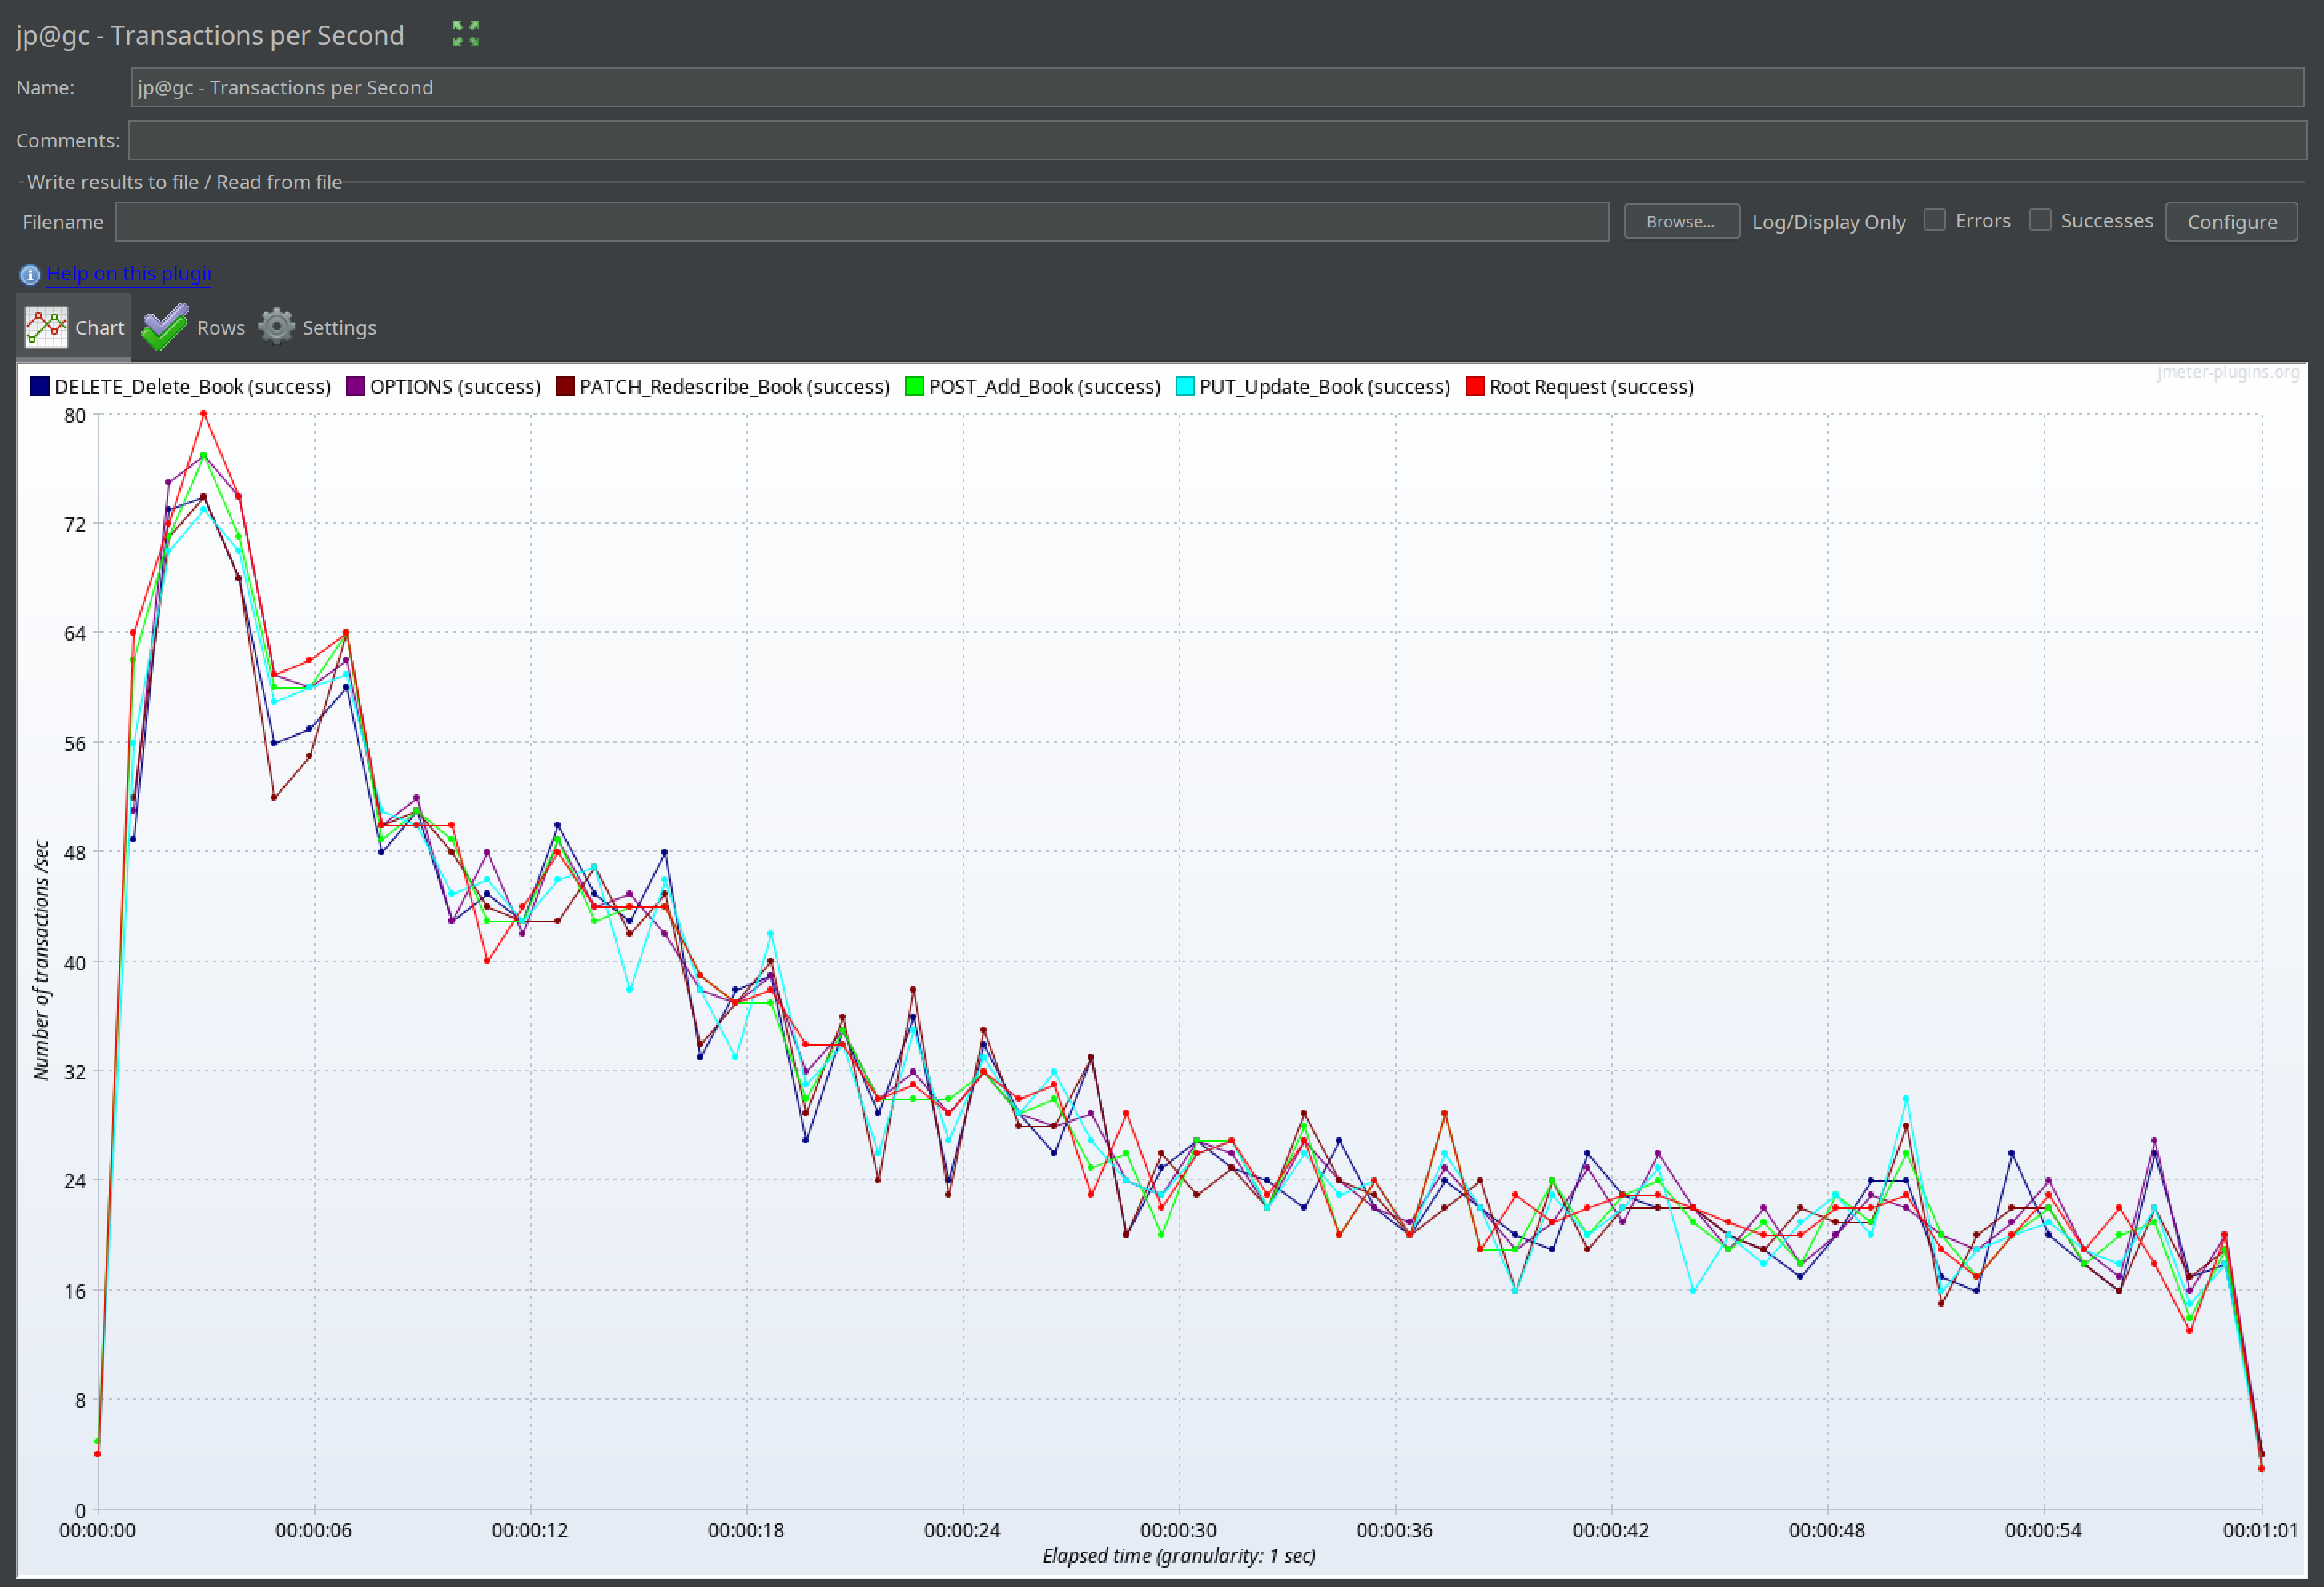
\includegraphics[width=0.65\textwidth]{../perfRuns/secondRun.png}
    \caption{\textbf{Transaction per Second Graph}}
\end{figure}

\subsection{Second Run}

\begin{figure}[H]
    \centering
    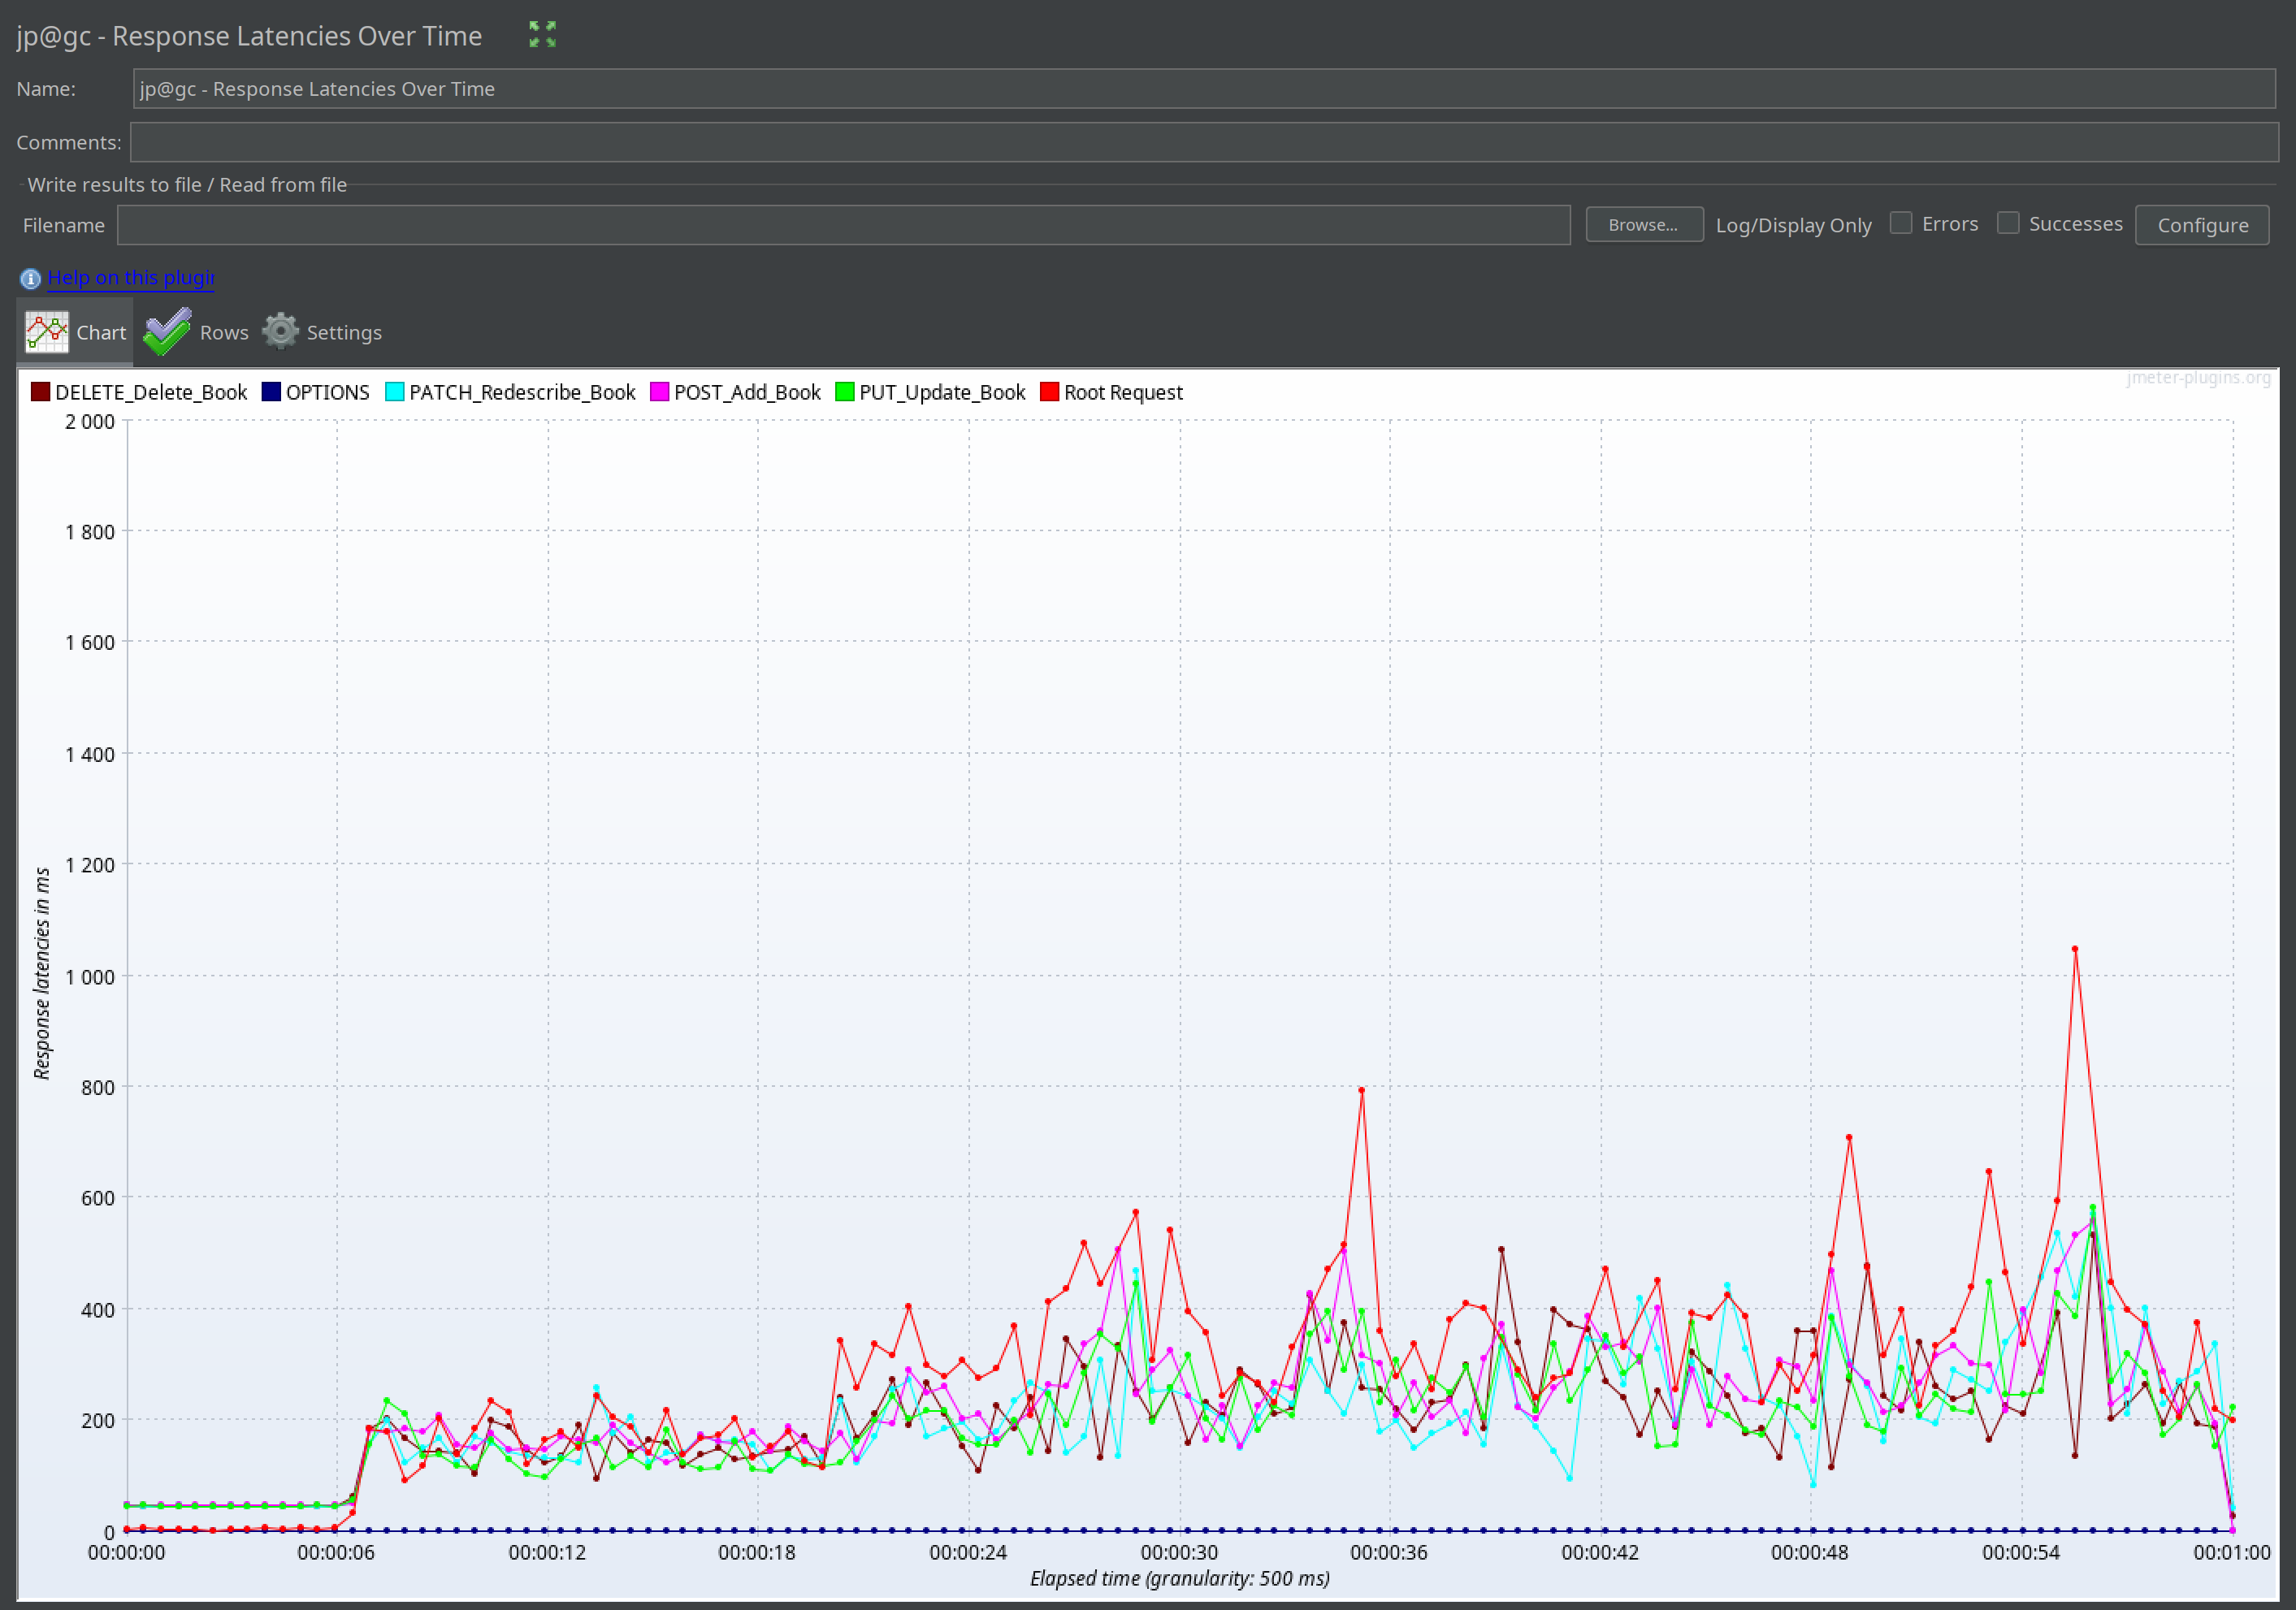
\includegraphics[width=0.65\textwidth]{../perfRuns2/thirdRunRespLatency.png}
    \caption{\textbf{Response Latency Graph}}
\end{figure}

\begin{figure}[H]
    \centering
    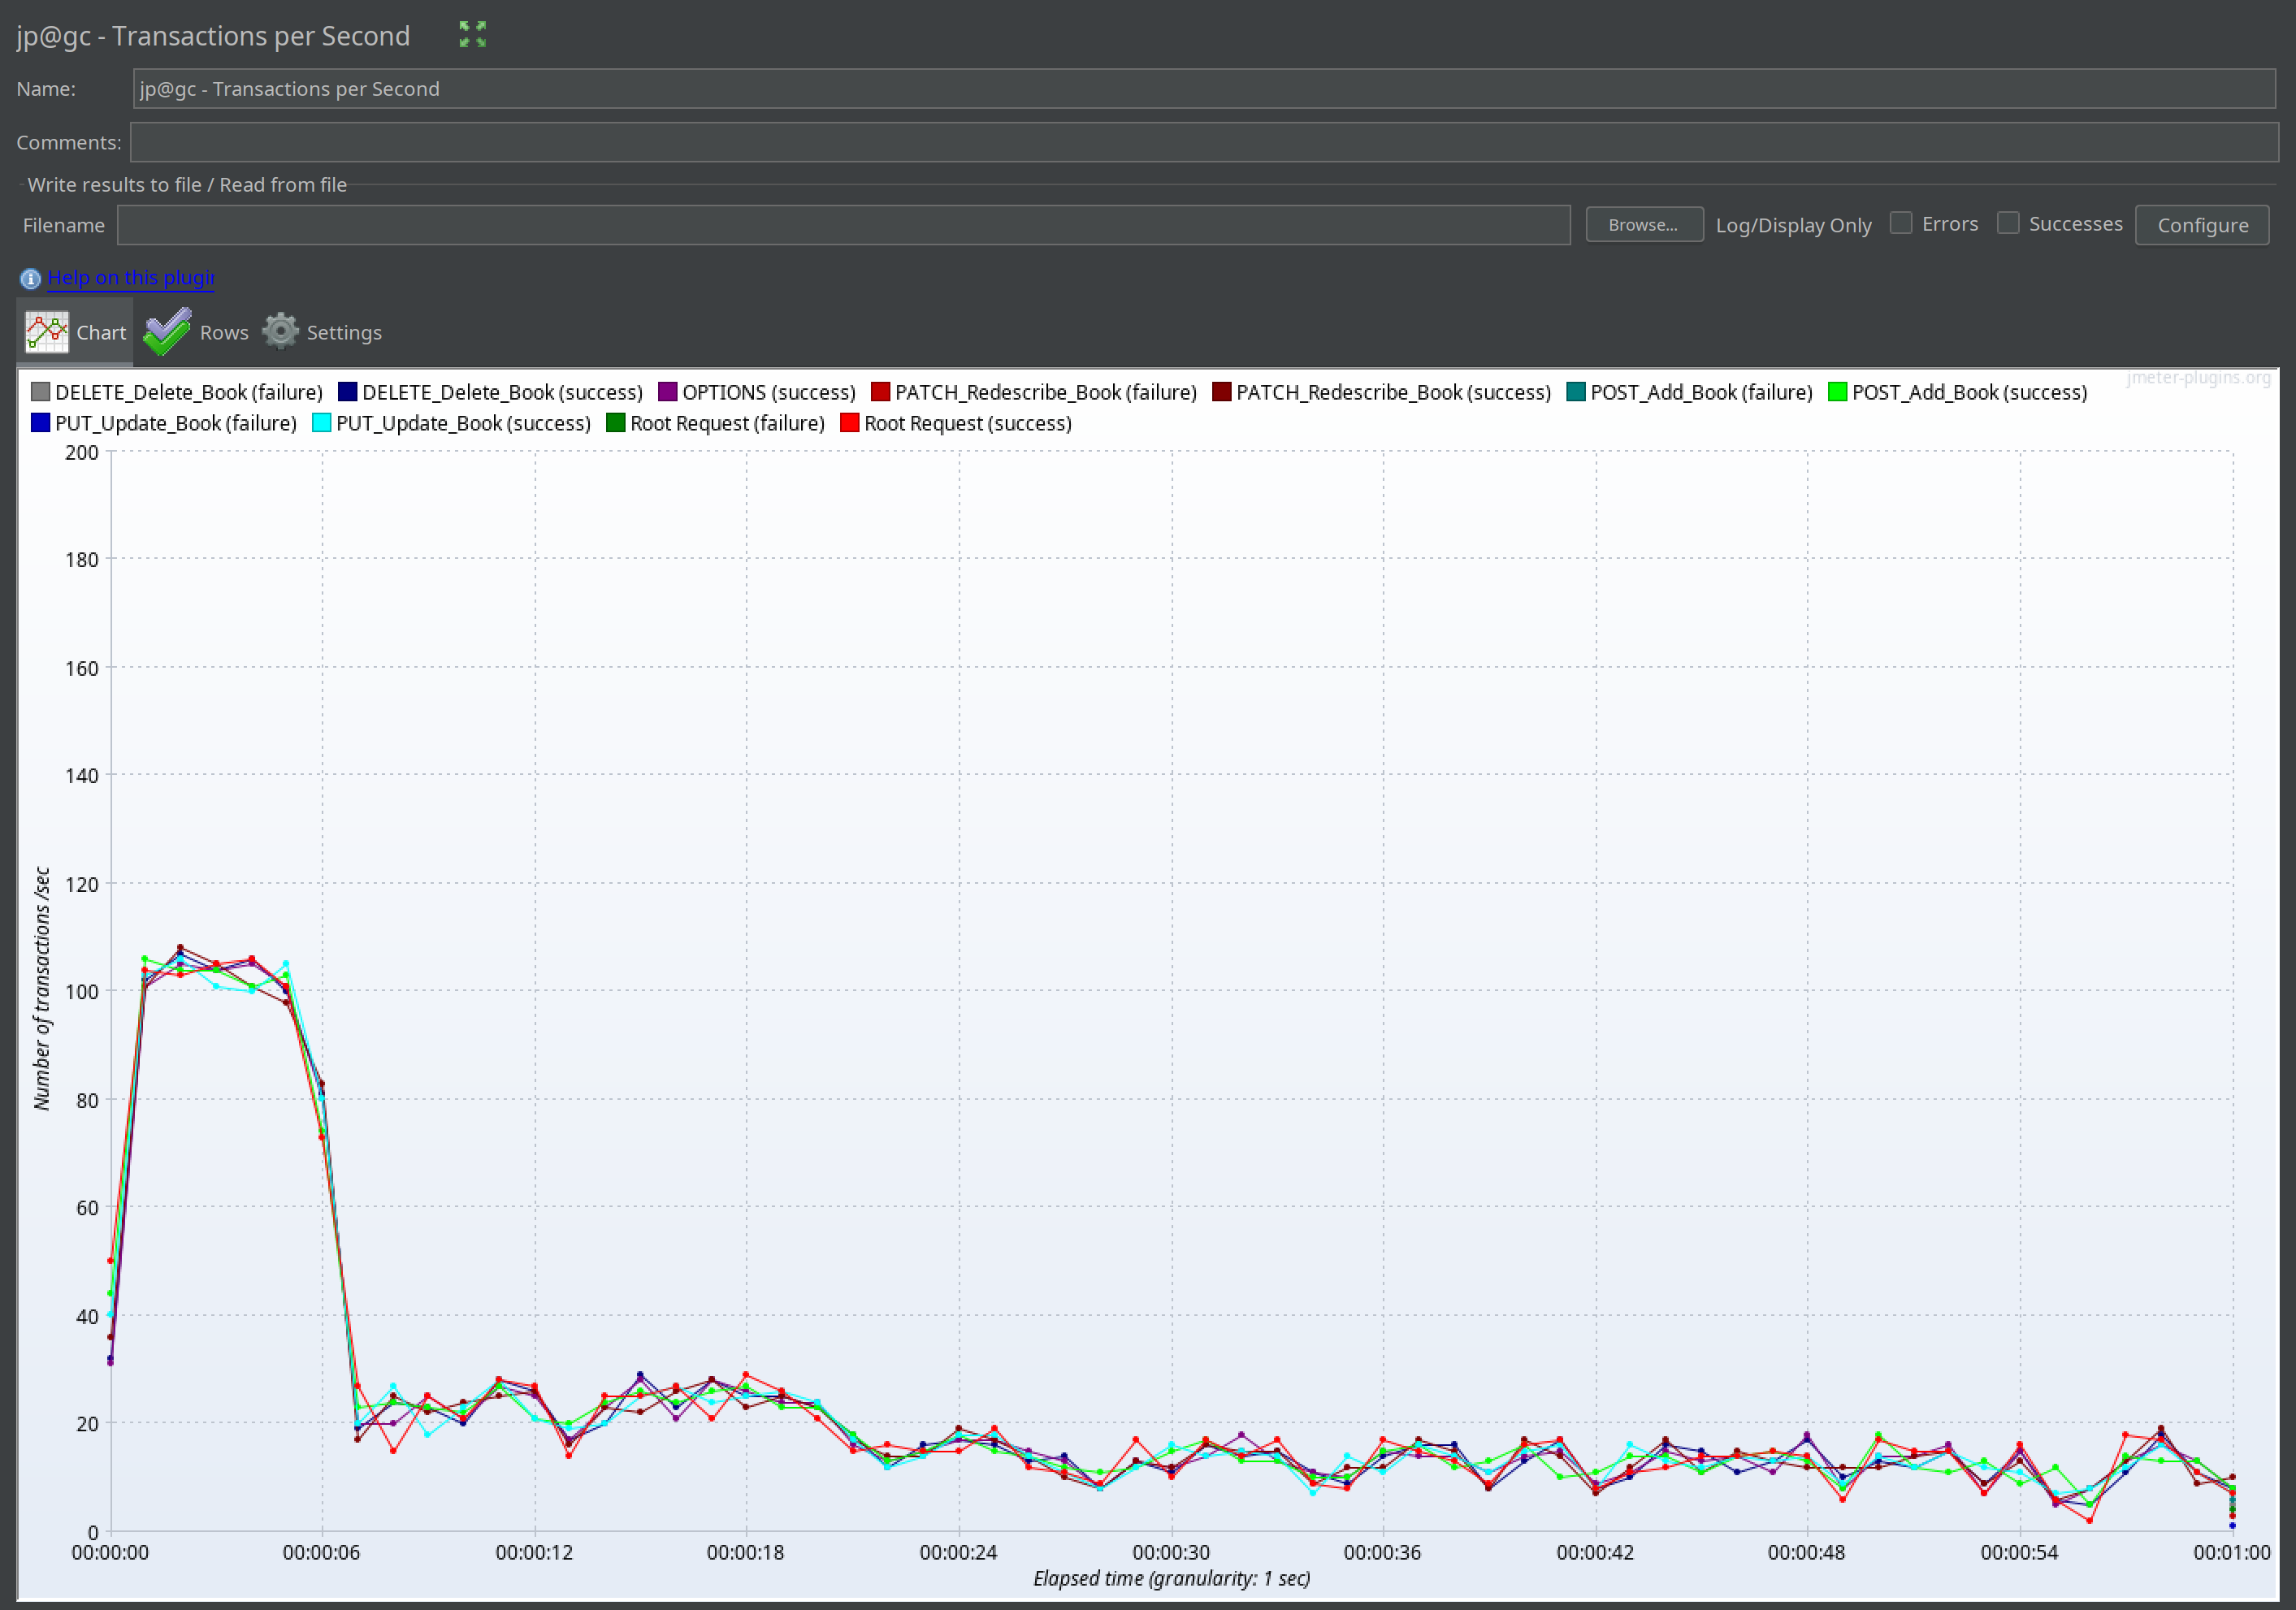
\includegraphics[width=0.65\textwidth]{../perfRuns2/thirdRunTrans.png}
    \caption{\textbf{Transaction per Second Graph}}
\end{figure}

\newpage

\section{Conclusion \& Future Work}

\par Performance testing is a collaborative effort where we measure our compliance with requirements, and business needs, ensuring
that information systems are able to perform on day to day business operations. Testing ensures that potential bugs, or performance bottlenecks
are accounted for and dealt with at due time, where it can significantly reduce costs, and aid with risk avoidance.

\newpage

% \nocite{becona2022}
\phantomsection
\printbibliography[heading=bibintoc]

\end{document}